\documentclass[11pt,a4paper]{article}
\usepackage[margin=25mm]{geometry}
\usepackage[T1]{fontenc}
\usepackage{newtxtext,newtxmath}
\usepackage{microtype,graphicx,booktabs,amsmath,array}
\usepackage[round,authoryear]{natbib}
\usepackage{xcolor,fancyhdr,caption}
\usepackage[colorlinks=true,linkcolor=black,citecolor=black,urlcolor=blue!45!black]{hyperref}
\hypersetup{pdftitle={What Should the Acid Leave Behind?},pdfauthor={Shivam Gupta},pdfsubject={History of fallout measurement, 1960-1961}}
\setlength{\parindent}{1.2em}\setlength{\parskip}{3pt}
\captionsetup{font=small,labelfont=bf}
\pagestyle{fancy}\fancyhf{}\fancyhead[L]{\small Gupta | Fallout measurements}\fancyhead[R]{\small Research manuscript}\fancyfoot[C]{\thepage}
\setlength{\headheight}{14pt}
\title{\LARGE What Should the Acid Leave Behind?\\[5pt]\Large Resin, Soil, and the Repair of Fallout Measurements, 1960--1961}
\author{Shivam Gupta\\\normalsize Independent Scholar, India\\\normalsize\href{mailto:shivam1720406@gmail.com}{shivam1720406@gmail.com}}
\date{16 October 2026}
\newcommand{\sr}{\ensuremath{^{90}\mathrm{Sr}}}
\newcommand{\unit}{\ensuremath{\mathrm{mCi}\,\mathrm{mi}^{-2}}}
\begin{document}
\maketitle
\begin{abstract}
In 1961, the US Atomic Energy Commission's Health and Safety Laboratory described acid extraction as a remedy for strontium-90 contamination inside fallout collectors. In the same quarterly report, incomplete acid extraction from soil remained a reason to question, but not yet correct, estimates of accumulated fallout. Why could leaving radioactive material behind validate one measurement and compromise another? This article reconstructs the two decisions through published laboratory reports and a reproducible analysis of sixteen paired soil measurements. The distinction depended on the provenance of the isotope, the intended measurement, and the credibility of the comparison procedure. Unused collectors supported a numerical correction and a change in resin processing; contaminated fusion facilities and the absence of replacement replicates impeded a comparable correction for soil. Recalculation gives a mean acid-to-fusion ratio of 86.62\%, identifies an unresolved discrepancy between the table and its summary range, and shows why a regression intercept did not establish a universal unextractable quantity. A constructive rounding check also reconciles apparently different residual sums of squares. The case locates the making of environmental data in selective dissolution, material supply, and the institutional capacity to repeat a test. Its contribution is a comparative history of correction and deferred correction, with an inspectable numerical record, rather than a new radiochemical technique or a retrospective exposure assessment.
\end{abstract}
\noindent\textbf{Keywords:} history of radiochemistry; nuclear fallout; environmental monitoring; material provenance; analytical uncertainty; reproducible history

\section{An isotope on both sides of the measurement}
The July 1961 \textit{Fallout Program Quarterly Summary Report} described an unwelcome persistence. Starting in July 1960, stainless-steel pots indicated declining strontium-90 deposition, while collectors using ion-exchange columns did not. Analyses of unused columns implicated the collecting material itself: radioactive strontium was present inside the resin and survived ordinary conditioning. HASL reported a subtraction of 0.24 millicuries per square mile for each column and, beginning with March 1961 collections, a change to acid extraction. The new treatment was intended to remove deposited fallout without releasing activity already bound inside the beads \citep[pp.~2--3]{hasl113}.

Later in the same volume, Edward Hardy discussed acid extraction from soil. Here, strontium-90 left behind was potentially part of the object being measured. An earlier comparison had suggested incomplete extraction, but the published results had not been corrected. A new set of sixteen comparisons remained difficult to interpret after the first fusion attempt was compromised by contamination in the furnace room. Further blind tests in a different facility were being prepared \citep[pp.~97--100]{hardysoil}. More complete dissolution promised a better comparison for soil, whereas it had made the resin measurement worse.

This conjunction is the article's starting point. It does not reveal a contradiction in chemistry: the materials, protocols, and analytical purposes differed. It reveals a historical problem in how measurements acquired authority. Both measurements concerned the same radionuclide and could be expressed as activity per unit area. Yet neither the isotope label nor the unit specified which activity should enter the result. That depended on whether a strontium atom belonged to the environmental material under investigation or to the apparatus used to investigate it.

The argument is that repair required two linked judgments. First, investigators had to distinguish the target from material introduced by the procedure. Second, they had to establish that the proposed comparison or correction had an adequate evidential basis. Resin contamination and soil extraction were therefore handled differently. In the former case, testing unused material supported a correction and a processing change. In the latter, an attempt to establish a more complete measurement was itself compromised, and the replacement analysis lacked a reproducibility study. The difference concerned the organization of evidence as much as the availability of an arithmetic adjustment.

A computational reconstruction makes that distinction more precise. It cannot rerun a 1961 assay, identify the unnamed soils, or establish an institution's private intentions. It can preserve the rows actually printed, distinguish several summaries that produce different percentages, and test the numerical implications of proposed loss models. It also makes it possible to separate a discrepancy that survives rounding from one that rounding can explain. These are necessary constraints on a history that uses laboratory numbers as evidence.

\section{Fallout histories and the scale of this intervention}
The global character of radioactive fallout, the political stakes of its measurement, and the constructed character of environmental data are well-established historical subjects. \citet{higuchi2018} shows how advisory bodies approached uncertainty from different commitments and concerns during the Eisenhower administration's test-ban deliberations. The implication for this study is methodological: numerical disagreement should not automatically be reduced either to a conflict between accurate and inaccurate science or to a direct expression of political allegiance. The practices that made a number credible require investigation.

\citet{chadarevian2024} compares Project Sunshine, United Nations data collection, and the St.~Louis Baby Tooth Survey as distinct ways of constructing the global dimension of strontium-90 contamination. That analysis also attends to differences in diet and calcium content across regions. A new study cannot plausibly claim that geographic comparability or nutritional normalization has escaped historical notice. The present article instead follows a particular radionuclide through two material settings within a laboratory publication: the manufactured collector and the sampled soil.

The institutions in these accounts were neither merely repositories of observations nor unchanging sources of authority. Herran's work on international radiation monitoring, discussed by de Chadarevian, places transnational surveillance within contested institutional arrangements \citep{herran2014,chadarevian2024}. \citet{creager2013} establishes the broader historical importance of radioisotopes as tools whose scientific and political lives were intertwined. These perspectives make a material problem inside a resin bead relevant to the history of environmental knowledge. It affected how activity could be assigned to a place and an interval before any wider synthesis could use it.

The intervention here is deliberately narrower than these histories. It joins HASL's account of its collector problem to Hardy's discussion of soil recovery, Ong's analysis of reproducibility, and Wilson's account of contractor quality control. Their juxtaposition permits a comparison between correction that was reported as implemented and correction that was explicitly deferred. The sixteen-soil reanalysis supplies an additional evidential layer: it tests which features of the published argument can be reconstructed from the printed table and which require qualifications.

Targeted searches combined the report numbers and authors with resin contamination, acid extraction, fusion, soil, fallout, reproducibility, and history. The directly relevant technical account was already published by HASL. No prior historical study of this particular comparison was located in the materials consulted. That bounded search result does not establish universal priority. The contribution is the comparative interpretation and its auditable reconstruction, not discovery of resin contamination or of incomplete chemical recovery.

\section{Sources, transcription, and the limits of the record}
\subsection{A public report as a record of work}
The principal source is HASL-113, issued on 1 July 1961 and reporting material available between March and June. It includes monitoring tables, procedural notes, interpretive contributions by named specialists, and a bibliography. HASL-105, issued in January 1961, provides a preceding account of the network, the division of work between HASL and contractors, and the publication of revisions \citep{hasl105,hasl113}. The 1962 UNSCEAR environmental-contamination annex supplies a contemporary international context for distinguishing environmental quantities and their routes through food chains \citep{unscear1962}.

These are published institutional accounts. They document what investigators were prepared to state publicly and how they justified particular interventions. They are not laboratory notebooks, correspondence with the resin manufacturer, or records of all unsuccessful tests. The date when a report described a discovery must not be silently substituted for the date when every participant first recognized it. Similarly, a published plan for new experiments does not establish that those experiments were completed or successful.

HASL-113 provides the scope of its collection network: forty sites in the United States and eighty-six outside it. Eighty-six of the 126 sites used funnels with ion-exchange columns, and four sites used both pots and columns. These are the report's network counts, not the result of a new census and not a count of independently affected assays. The report does not supply enough information about resin lots and their distribution to attribute the same contamination history to every column result \citep[pp.~2--3]{hasl113}.

\subsection{The sixteen-soil dataset}
The numerical corpus is the complete table on printed page 99 of HASL-113, not a selection of conspicuous residuals. Each row preserves its published site identifier, sampling depth, acid-extraction value, fusion value, and rounded percentage. All measurements are in millicuries of strontium-90 per square mile. The identifiers do not provide geographic names. Depths range from two to nine inches. Hardy states that these sixteen samples were selected from 125 soils collected in 1959 to span locations and low, medium, and high concentrations \citep[p.~97]{hardysoil}. They are therefore not a probability sample of the world, and their unweighted mean is not a global recovery estimate.

Text extraction was checked against the page image, including site 10 and the summary below the table. The dataset preserves both the row and the inconsistent summary rather than changing either to agree with the other. Site 10 is printed as 14 for HCl extraction, 21 for fusion, and 67\%. The summary gives a range of 78--101\%. That is an issue in the source itself, not an optical-character-recognition substitution. This study does not identify which historical entry, if any, should have been different.

The analysis script recomputes ratios and least-squares fits, performs sixteen leave-one-site-out fits, constructs a numerical witness for the effect of rounding, and evaluates two simple loss models under explicit tolerance assumptions. An independent linear-programming implementation checks the compatibility calculations. These checks validate the reconstruction and calculations; they do not independently validate the original radiochemical measurements.

\begin{table}[t]
\centering\small
\caption{The evidential roles of the principal source passages. Page numbers refer to the reports' printed pagination.}
\begin{tabular}{p{.19\linewidth}p{.24\linewidth}p{.47\linewidth}}
\toprule
Source & Passage & What it can establish\\\midrule
HASL-105 & pp.~2--3 & Network organization, contractor analyses, and an explicit process for publishing revisions.\\
HASL-113 & pp.~2--3 & Reported collector discrepancy, unused-column tests, subtraction, and processing change.\\
Ong in HASL-113 & pp.~75--80 & A distinction between counting error and reproducibility, based on paired analyses.\\
Wilson in HASL-113 & pp.~81--84 & Contractor standards, replicates, and reagent blanks as different quality checks.\\
Hardy in HASL-113 & pp.~97--100 & Soil comparison, compromised first fusion attempt, replacement analysis, and planned tests.\\
UNSCEAR 1962 & Annex F, Part II, paras.~17--20 & Contemporary distinction between chemical extraction, availability, and environmental transfer.\\\bottomrule
\end{tabular}
\label{tab:sources}
\end{table}

\section{When the collector became a source}
The network relied on material and organizational substitutions. Local personnel or cooperating scientists collected samples; HASL or private laboratories analyzed them. HASL-105 describes open pots, funnels attached to ion-exchange columns, and rain gauges aboard weather ships. Contractor collections could include duplicate samples and a broader set of radionuclides \citep[p.~2]{hasl105}. A map of stations thus concealed several different routes from exposure to reported activity.

The persistence of a reading acquired significance through comparison. According to HASL-113, pots and columns began to diverge in July 1960: declining pot readings were not matched by the columns. The comparison did not, by itself, identify a cause. It made a difference between collection methods visible. The next evidential move was to analyze columns that had not been exposed to environmental collection. Their activity implicated a contribution that could not be assigned to the period's deposited fallout \citep[pp.~2--3]{hasl113}.

The report attributed approximately seventeen disintegrations per minute per column, expressed as 0.24 \unit, to strontium-90 bound within the resin during polymerization. That attribution is the laboratory's published explanation. The report contains no manufacturing records that would permit an independent reconstruction of the event. It does, however, specify why ordinary conditioning did not remove the contribution and why the analytical procedure made the problem consequential. Ashing followed by sodium-carbonate fusion rendered the resin soluble and made its internal activity indistinguishable from collected fallout \citep[p.~3]{hasl113}.

The remedy had a retrospective and a prospective component. The report states that affected column results were corrected by subtracting the specified amount for each column. For new collections beginning in March 1961, acid extraction was intended to release the activity acquired during exposure while leaving the resin's inherent contribution inside the bead. A resin free of the reported contamination had also been obtained for future use. A correction to published values, a change in laboratory processing, and a change in material supply were distinct interventions. They should not be compressed into a single date when the collector was simply ``fixed.''

The quantity 0.24 also requires its denominator. A correction per column is not automatically a correction per table row. HASL-113 states that, starting with May and June 1960, monthly collections were combined for analysis on a two-month basis at most sites because activity levels had fallen \citep[pp.~2--3]{hasl113}. Applying one subtraction to every row in a digitized table would therefore require information about how many columns contributed to each reported analysis, which material was implicated, and whether the value had already been corrected. The present reconstruction does not perform such a blanket subtraction.

The argument is not that greater dissolution is generally undesirable. Dissolving all of the resin was a problem because the resin contained activity outside the specified environmental target. Acid extraction was valuable precisely because it was selective. The validity of the reading depended on a material distinction that disappeared when everything was rendered soluble.

\begin{figure}[t]
\centering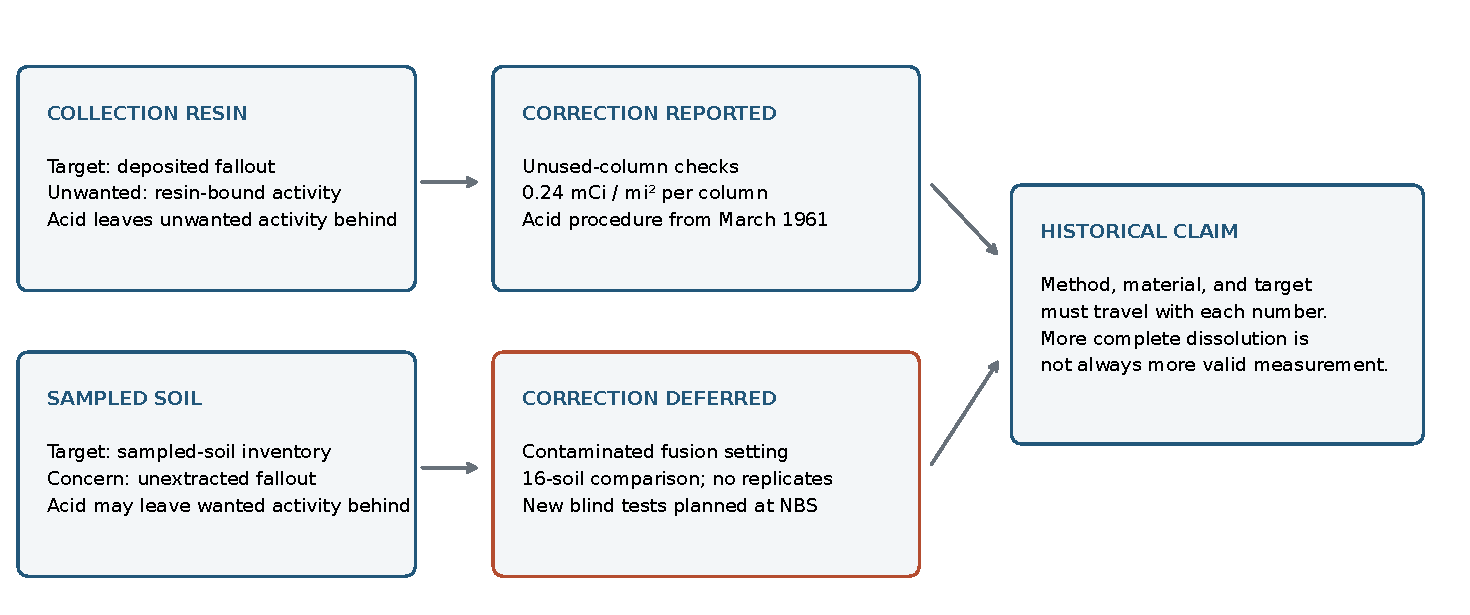
\includegraphics[width=\linewidth]{../figures/two_extractions.pdf}
\caption{Two roles for selective extraction in HASL-113. The diagram reconstructs the report's stated target and problem in each setting; it does not imply identical acid protocols or independently verified chemical recoveries. Sources: HASL-113, pp.~2--3; Hardy, pp.~97--100.}
\label{fig:roles}
\end{figure}

\section{When the comparison procedure also needed repair}
For soil, the objective described by Hardy was to document accumulated fallout. The acid method was treated as adequate for this material balance, with residual activity assumed negligible. That was an assumption about completeness relative to a specified target. It was not merely a statement that the procedure produced reproducible readings \citep[p.~97]{hardysoil}.

Hardy's retrospective account reports that nine earlier comparisons had yielded an average extraction of 84\%, conditional on treating fusion as a total measurement. Nonetheless, earlier acid-extraction results had not been corrected. Sixteen soils collected in 1959 were subsequently selected for further comparison. Their first fusion took place at the Soil Survey Laboratory in Beltsville. After crushing and blending the melts, duplicate aliquots were sent to HASL without identities that would reveal the matching pairs. Decoding revealed poor reproducibility and levels considered theoretically impossible. A contaminated furnace room was subsequently identified \citep[p.~97]{hardysoil}.

This was not an absence of quality control. The attempted blind comparison was part of the process by which a problem was exposed. Nor can the fusion readings be treated as an unproblematic external truth. The procedure proposed to test the acid method could introduce its own unwanted activity. The two cases therefore shared a difficulty more specific than generic measurement error: an operation intended to make the radionuclide accessible could also make extraneous radionuclide enter the result.

New identified aliquots of the original soils were sent to HASL, where smaller samples were fused. Hardy explicitly states that time and facilities were unavailable for studying reproducibility at this stage. Those replacement results appear in the sixteen-row table. They are the results reconstructed here; the compromised first-run duplicate measurements are not printed in that table and cannot be recovered from it. The report describes a further set of fusions being prepared in a radiation-free area at the National Bureau of Standards, with blind replicates planned. It closes by connecting those tests to a future decision about correcting extraction results \citep[pp.~97--98]{hardysoil}.

The surrounding contributions explain why precision was an active concern. Ong distinguishes the Poisson counting error accompanying an individual result from the reproducibility of the measuring process. His analysis of 180 soil pairs, collected between 1956 and 1959, models the absolute difference between repeated analyses rather than treating the counting error as the complete uncertainty \citep[pp.~75--76]{ong1961}. Wilson's description of a contractor laboratory separates counter calibration, replicate analysis, and contamination checks using blanks. His combined validity estimate is conditional on achieving a specified counting precision \citep[pp.~81--82]{wilson1961}. These accounts should not be imported wholesale as error bars for Hardy's replacement fusions. They show, instead, that the report itself distinguished several objects of quality control.

An unused resin column addressed a different question from a reagent blank or a duplicate aliquot. The column could expose activity already present in the collector. A blank followed reagents and processing. A replicate tested repeatability conditional on the material and operations shared by the measurements. Good performance on one did not logically establish good performance on the others. HASL's report assembled these checks without making them interchangeable.

\section{What the sixteen printed comparisons support}
\subsection{Ratios, ranges, and different averages}
Write $H_i$ for the printed HCl value and $F_i$ for the fusion value. The reconstructed percentage is $100H_i/F_i$. Fourteen of the sixteen acid readings are below their fusion counterparts; two are slightly above. The unweighted mean percentage is 86.62, with a sample standard deviation of 8.81 percentage points. This is descriptive dispersion among selected soils, not uncertainty on a representative global mean. The ratio of the sums is different: $100(797/898)=88.75$. It weights each ratio by its fusion value. Neither quantity is an area-weighted estimate of the Earth's inventory.

The mean rounds to the report's printed 87\%. The reconstructed dispersion is not identical to the printed 8, and the table's actual minimum is 66.67\%, not 78\%. The range discrepancy is particularly clear because the row itself prints 67\%. Even allowing both concentrations in that row to have been rounded to the nearest integer, its largest possible ratio is $100(14.5/20.5)=70.73\%$. Rounding of those two values cannot lift the row into a range beginning at 78\%. This establishes a documentary inconsistency; it does not establish whether the row, summary, or an underlying calculation was mistaken.

\begin{figure}[t]
\centering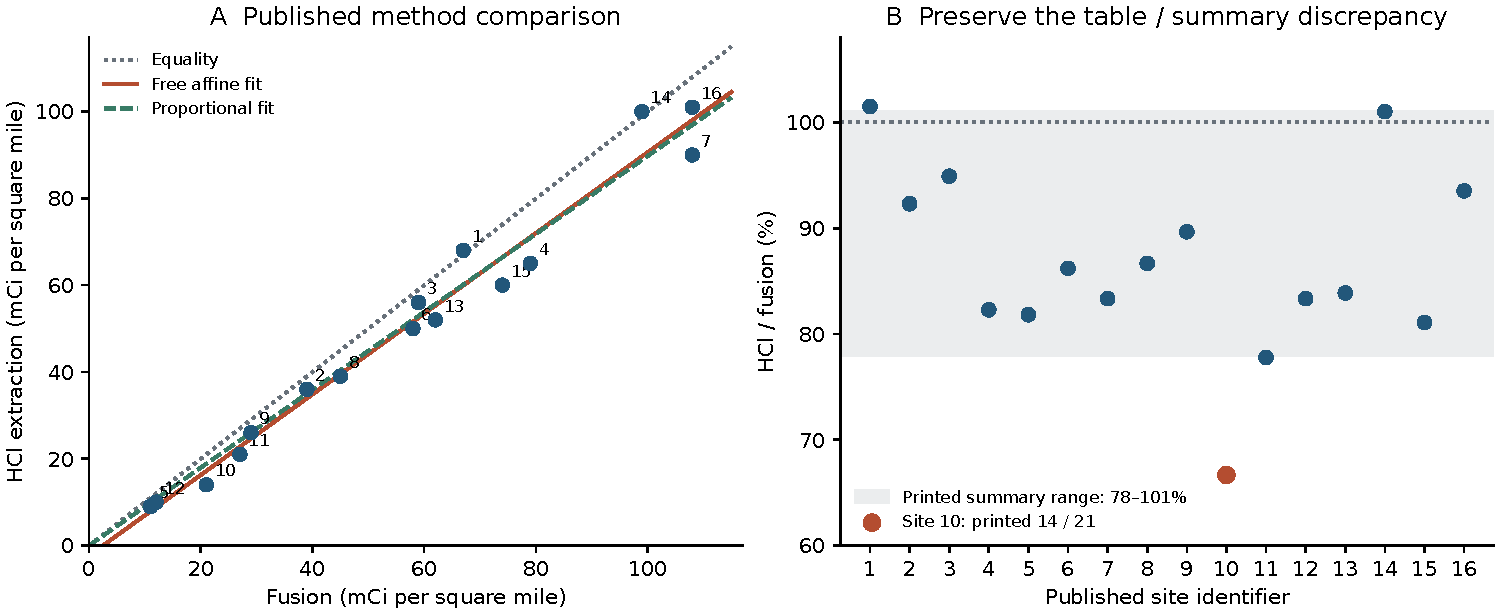
\includegraphics[width=\linewidth]{../figures/soil_comparison.pdf}
\caption{Reconstruction of all sixteen printed comparisons. A: equality, free affine regression, and a fitted proportional relation. Labels are the source's site identifiers. B: individual ratios against the printed summary range. The shaded range is a source assertion, not an uncertainty interval. Source: Hardy, HASL-113, p.~99.}
\label{fig:soil}
\end{figure}

\subsection{An intercept is not a recovered physical reservoir}
Hardy discusses a least-squares line whose intersection with the horizontal axis is a little over two millicuries per square mile. He considers the implication of a constant unextractable amount but qualifies it in light of analytical error and dispersion \citep[p.~98]{hardysoil}. The printed pairs reproduce the approximate intercept:
\begin{equation}
\widehat H=-2.3250+0.9290F,\qquad F\big|_{\widehat H=0}=2.5028.
\label{eq:ols}
\end{equation}
This is a fitted relation over the observed values. An exactly constant absolute loss, $H=F-d$, additionally requires a slope of one. Its fitted loss is $d=6.3125$, not 2.5028. Confusing the free line's horizontal intercept with a demonstrated fixed reservoir would erase that distinction.

Table~\ref{tab:models} compares three elementary descriptions. Their least-squares fits are computed from the published numbers, without claiming that fusion is error-free. The free affine model has the lowest in-sample residual sum of squares, as expected when an extra parameter is available. That advantage does not persist in the leave-one-site-out prediction summary. These prediction errors are a finite-data diagnostic, not an estimate of performance on a randomly sampled future soil population. The affine horizontal intercept also varies from 1.28 to 3.78 when individual sites are omitted.

\begin{table}[t]
\centering\small
\caption{Descriptive models fitted to the sixteen printed pairs. SSE has squared activity-per-area units; held-out RMSE has \unit\ units. Fusion is a comparison measurement, not an independently known truth.}
\begin{tabular}{lrrr}
\toprule
Model & Fitted parameter(s) & SSE & Leave-one-out RMSE\\\midrule
$H=a+bF$ & $a=-2.3250,\ b=0.9290$ & 371.47 & 5.667\\
$H=rF$ & $r=0.89725$ & 391.76 & 5.583\\
$H=F-d$ & $d=6.3125$ & 449.44 & 5.653\\\bottomrule
\end{tabular}
\label{tab:models}
\end{table}

One apparent failure to reproduce the original calculation has a constructive resolution. Hardy gives 359 for the residual sum of squares, whereas Equation~\ref{eq:ols} yields 371.47. The concentrations were printed as integers. Let $\widehat H_i$ be the fitted values and $e_i=H_i-\widehat H_i$. The values
\begin{equation}
H_i^*=\widehat H_i+\sqrt{359/371.47224}\,e_i
\label{eq:witness}
\end{equation}
retain the same least-squares coefficients and give a residual sum of squares of 359. Each differs from its printed value by at most 0.176, well inside half a printing unit. Thus an underlying dataset compatible with the printed rounding can reproduce 359. This witness does not identify the original unrounded measurements; it shows why the residual discrepancy must not be reported as a demonstrated historical calculation error.

\subsection{Sensitivity to an explicit analytical tolerance}
The report discusses ten-percent analytical error as a caution. That statement does not specify independent Gaussian errors or a confidence region for these sixteen pairs. The following exercise therefore treats a common relative tolerance $\epsilon$ as a declared sensitivity assumption. For each measurement, the unknown comparison value may lie between $(1-\epsilon)$ and $(1+\epsilon)$ times the printed value. The exercise asks whether a simple model could satisfy every pair simultaneously within that allowance. It neither assigns probabilities nor proves a chemical mechanism.

For a common extraction fraction $0\leq r\leq1$, feasibility is equivalent to a nonempty intersection
\begin{equation}
[0,1]\ \cap\ \bigcap_i
\left[\frac{H_i}{F_i}\frac{1-\epsilon}{1+\epsilon},
\frac{H_i}{F_i}\frac{1+\epsilon}{1-\epsilon}\right].
\label{eq:prop}
\end{equation}
For a fixed additive loss $d\geq0$, the corresponding intersection is
\begin{equation}
[0,\infty)\ \cap\ \bigcap_i
\left[(1-\epsilon)F_i-(1+\epsilon)H_i,
(1+\epsilon)F_i-(1-\epsilon)H_i\right].
\label{eq:add}
\end{equation}
These follow directly from interval arithmetic; no new estimation method is claimed. At ten percent the common-fraction intersection is empty, with lower endpoint 0.83039 above upper endpoint 0.81481. The additive intersection is nonempty, $d\in[3.5,4.0]$. The smallest uniform tolerances for feasibility are 10.47\% for the fraction model and 9.09\% for the additive model. Removing site 10 makes the fraction model feasible at ten percent. This is a sensitivity result about an influential row, not a justification for deleting it.

The analysis incorporates the two measurements symmetrically as uncertain quantities, but the choice of uniform tolerance is still an assumption. Site-specific uncertainties and covariance are unavailable. Compatibility of the additive model under this allowance does not corroborate a fixed unextractable amount; incompatibility of the fraction model at exactly ten percent does not reject a stochastic model of proportional recovery. Moving the allowance by less than half a percentage point changes the latter verdict. The calculation gives a precise reason to retain Hardy's caution rather than upgrade a suggestive line into a universal correction.

\begin{figure}[t]
\centering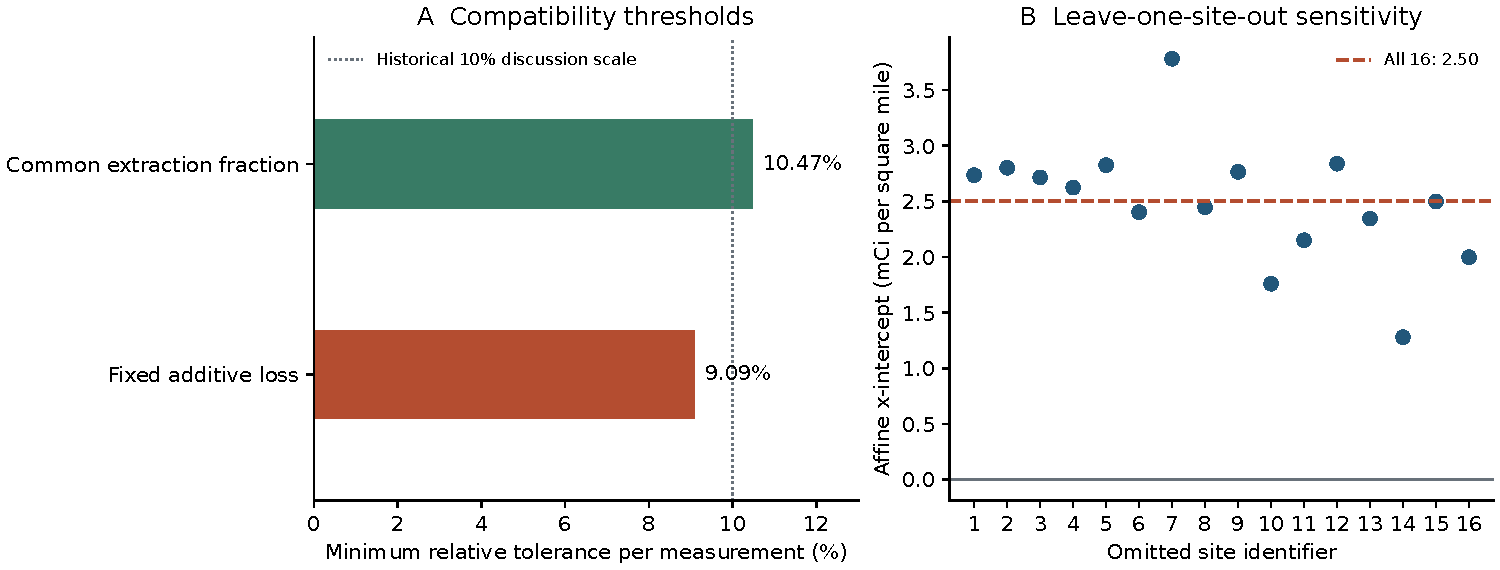
\includegraphics[width=\linewidth]{../figures/model_sensitivity.pdf}
\caption{Two finite-data sensitivity checks. A: minimum componentwise relative tolerance under the stated model, with ten percent shown for comparison to the report's discussion. These are not confidence levels. B: the affine line's horizontal intercept after each single-site omission. All sixteen omissions are shown; no site is removed from the primary analysis.}
\label{fig:sensitivity}
\end{figure}

\section{Correction, provenance, and institutional capacity}
Reading the episodes together changes the historical question. It is insufficient to ask whether a laboratory extracted all the strontium-90. For the manufactured collector, a more complete dissolution could produce a less appropriate estimate of environmental deposition. For a sampled-soil inventory, incomplete dissolution could omit part of the intended quantity. The relationship between chemical completeness and evidential validity reversed because the target and the provenance of the activity differed.

This was not simply an opposition between nature and an artificial contaminant. Fallout was itself artificial, and the same isotope could be found in environmental soil, collected precipitation, and manufactured resin. Its nuclear identity could not tell the analyst which material history should count. The relevant boundary ran between activity attributable to the stated target and activity entering by another route. Blank design and sample preparation made that distinction operational.

The published difference between correction and deferral also shows why uncertainty cannot be represented only by a wider numerical interval. HASL reported an unused-material test and a specified subtraction for resin. Hardy's soil comparison depended on a reference procedure whose first implementation had failed, followed by replacement analyses without the desired reproducibility check. An adjustment was numerically conceivable: dividing by a chosen recovery fraction would be trivial. Authorizing it across earlier results required additional evidence about the reference and the range of materials to which it could apply.

Time, facilities, and institutional cooperation entered that authorization. Beltsville prepared the first fusions; HASL analyzed the aliquots and replacements; NBS was to provide a different setting for further work. The declared lack of time and facilities for replacement replicates was therefore consequential to what could be said about accumulated fallout. It was not an incidental logistical detail to be removed from a clean account of a method comparison. At the same time, this published explanation alone cannot establish a general shortage of resources across HASL or a political decision to suppress a correction.

The report's multiple quality-control contributions make a simple narrative of concealment particularly inadequate for this case. It printed the contamination account, the compromised comparison, limitations of uncertainty reporting, and a plan for additional tests. Publication was part of the repair process. That observation does not absolve the larger nuclear establishment of the political problems documented by historians of fallout. It identifies a local evidential practice that cannot be inferred directly from those broader problems.

There is also a practical consequence for the digital afterlife of these records. A database that retains only station, month, isotope, and value can place already-corrected results beside uncorrected ones, flatten a pooled interval into a month, or treat an acid-soluble fraction as a total inventory. A minimally adequate record should retain the source edition and page, sampled material, collection interval, collector and preparation method, correction status, and the intended environmental quantity. ``Unknown'' should remain a possible value. An absent lot history must not become a confident batch attribution.

The accompanying code demonstrates one part of that practice. It stores reported values separately from recalculated summaries, publishes the source discrepancy without repairing it by assumption, and distinguishes a rounding-compatible residual from an irreconcilable printed range. Such a workflow can support archival and environmental-data services. The present study has not measured a market, validated a commercial product, or established a patentable radiochemical invention. Its practical value lies in keeping the conditions of historical measurements available for inspection.

\section{Scope, limitations, and conclusion}
This is a comparison within a small public documentary corpus. It does not determine how much every resin batch was contaminated, which laboratories adopted the revised processing when, or how later tests resolved the soil question. The sample identifiers cannot be used for geographic inference, and varying collection depths prevent a straightforward interpretation as a common soil horizon. Fusion is a reported comparison method whose limitations are central to the story. The calculations are therefore not new estimates of global fallout, dietary intake, biological availability, or health effects.

The final distinction matters historically as well as technically. UNSCEAR's contemporary discussion separates extraction procedures and the availability of strontium and calcium to plants \citep[Annex F, Part II, paras.~17--20]{unscear1962}. Total sampled-soil activity, an acid-extractable fraction, and transfer into food are different objects. The fact that this article reconstructs an inventory-oriented comparison does not authorize its recovery ratios to be inserted into a dietary or exposure calculation.

Within those limits, the sources establish a substantive result. HASL's published program repaired measurements by distinguishing the material history of the isotope from its chemical identity, and it made different decisions about correction when the supporting experiments had different credibility. The sixteen-soil reconstruction supports a general tendency toward lower acid readings while preserving the instability of any universal correction. Its source audit also demonstrates that numerical disagreement itself has to be investigated: the printed range conflicts with a row, whereas the published residual can be reconciled with unprinted precision.

The episode offers a history of environmental monitoring in which collecting more places and detecting smaller activities were only part of the work. An environmental number also required a defensible account of what the laboratory should leave behind, what it should bring into solution, and which experiment could establish the difference.

\section*{Data and code availability}
The transcription, analysis, tests, figures, source manifest, and manuscript source are available at \url{https://github.com/shi1720/fallout-extraction-history}. All numerical results reported as new calculations are generated from the sixteen printed pairs. Source scans are linked rather than redistributed. The artifact includes a constructive rounding witness and complete single-site sensitivity results.

\begin{thebibliography}{99}
\bibitem[Creager(2013)]{creager2013} Creager, Angela N.~H. 2013. \textit{Life Atomic: A History of Radioisotopes in Science and Medicine}. Chicago: University of Chicago Press. \url{https://press.uchicago.edu/ucp/books/book/chicago/L/bo16382130.html}.
\bibitem[de Chadarevian(2024)]{chadarevian2024} de Chadarevian, Soraya. 2024. ``Collecting data on a global scale: from local to international and back again.'' \textit{Statistique et soci\'et\'e} 12(3). \href{https://doi.org/10.4000/13pbe}{doi:10.4000/13pbe}.
\bibitem[Hardy(1961)]{hardysoil} Hardy, E. 1961. ``Comparison Between HCl Extraction and Fusion Method for Determining Strontium-90 in Soil.'' In \textit{HASL-113}, 97--100. See Hardy, Rivera, and Frankel (1961b).
\bibitem[Hardy et~al.(1961a)]{hasl105} Hardy, Edward P., Jr., Joseph Rivera, and Robert Frankel, preparers. 1961a. \textit{Health and Safety Laboratory Fallout Program Quarterly Summary Report (September 1, 1960 through December 1, 1960)}. HASL-105. New York: US Atomic Energy Commission, 9 January. \url{https://digital.library.unt.edu/ark:/67531/metadc13063/}.
\bibitem[Hardy et~al.(1961b)]{hasl113} Hardy, Edward P., Jr., Joseph Rivera, and Robert Frankel, preparers. 1961b. \textit{Health and Safety Laboratory Fallout Program Quarterly Summary Report (March 1, 1961 through June 1, 1961)}. HASL-113. New York: US Atomic Energy Commission, 1 July. \url{https://digital.library.unt.edu/ark:/67531/metadc13065/}.
\bibitem[Herran(2014)]{herran2014} Herran, N\'estor. 2014. ```Unscare' and Conceal: The United Nations Scientific Committee on the Effects of Atomic Radiation and the Origin of International Radiation Monitoring.'' In Simone Turchetti and Peder Roberts, eds., \textit{The Surveillance Imperative: Geosciences during the Cold War and Beyond}, 69--84. New York: Palgrave Macmillan. \href{https://doi.org/10.1057/9781137438744_4}{doi:10.1057/9781137438744\_4}. Discussed here through de Chadarevian (2024).
\bibitem[Higuchi(2018)]{higuchi2018} Higuchi, Toshihiro. 2018. ``Epistemic frictions: radioactive fallout, health risk assessments, and the Eisenhower administration's nuclear-test ban policy, 1954--1958.'' \textit{International Relations of the Asia-Pacific} 18(1): 99--124. \href{https://doi.org/10.1093/irap/lcx024}{doi:10.1093/irap/lcx024}.
\bibitem[Ong(1961)]{ong1961} Ong, Long D.~Y. 1961. ``Reproducibility of Analysis of Soils for Strontium-90.'' In \textit{HASL-113}, 75--80. See Hardy, Rivera, and Frankel (1961b).
\bibitem[UNSCEAR(1962)]{unscear1962} United Nations Scientific Committee on the Effects of Atomic Radiation. 1962. ``Annex F: Environmental Contamination.'' In \textit{Report of the United Nations Scientific Committee on the Effects of Atomic Radiation}. General Assembly Official Records, Seventeenth Session, Supplement 16, A/5216. New York: United Nations. \url{https://www.unscear.org/unscear/uploads/documents/publications/UNSCEAR_1962_Annex-F.pdf}.
\bibitem[Wilson(1961)]{wilson1961} Wilson, C.~R. 1961. ``Internal Quality Control for Strontium-90 Analysis in the NSEC (Nuclear Science \& Engineering Corporation) Low-Level Radioactivity Laboratory.'' In \textit{HASL-113}, 81--84. See Hardy, Rivera, and Frankel (1961b).
\end{thebibliography}

\appendix
\section{The complete transcribed comparison}
\begin{table}[h]
\centering\small
\caption{All values as printed on HASL-113, p.~99. Depth is in inches; method values are in \unit. The last column is the printed rounded percentage.}
\begin{tabular}{rrrrr}\toprule
Site & Depth & HCl & Fusion & Percent\\\midrule
1&0--6&68&67&101\\2&0--6&36&39&92\\3&0--6&56&59&95\\4&0--7&65&79&82\\5&0--8&9&11&82\\6&0--5&50&58&86\\7&0--8&90&108&83\\8&0--2&39&45&87\\9&0--6&26&29&90\\10&0--8&14&21&67\\11&0--9&21&27&78\\12&0--6&10&12&83\\13&0--8&52&62&84\\14&0--8&100&99&101\\15&0--8&60&74&81\\16&0--8&101&108&94\\\bottomrule
\end{tabular}
\end{table}
\noindent Printed summary: average 87, standard deviation 8, range 78--101. These source assertions are retained without silently harmonizing them with the rows.

\section{Compatibility calculations and independent checks}
For the proportional model, let the latent values satisfy $h_i=rf_i$ and the two relative-tolerance intervals. For fixed $r$, $rf_i$ ranges from $r(1-\epsilon)F_i$ to $r(1+\epsilon)F_i$. Its intersection with the interval for $h_i$ is nonempty precisely when the lower endpoint in Equation~\ref{eq:prop} is no greater than $r$, and $r$ is no greater than the upper endpoint. Since latent values for different rows are unconstrained across rows, intersecting those conditions proves necessity and sufficiency.

For the additive model $h_i=f_i-d$, the differences of the two measurement intervals fill exactly the interval in Equation~\ref{eq:add}. Intersecting across rows and with $d\geq0$ proves necessity and sufficiency. If $q_i=H_i/F_i$, the smallest proportional tolerance is
\[
\epsilon_{\rm prop}=\max\!\left\{0,\ \frac{\sqrt{q_{\max}/q_{\min}}-1}{\sqrt{q_{\max}/q_{\min}}+1},\ \max_i\frac{H_i-F_i}{H_i+F_i}\right\}.
\]
Writing $D_i=F_i-H_i$ and $S_i=F_i+H_i$, the smallest additive tolerance is
\[
\epsilon_{\rm add}=\max\!\left\{0,\ \max_{i,j}\frac{D_i-D_j}{S_i+S_j},\ \max_i\frac{-D_i}{S_i}\right\}.
\]
The expressions include the physical constraints $r\leq1$ and $d\geq0$. All printed inputs are positive. The computer implementation checks the closed forms and interval tests against an independently formulated linear program with explicit latent variables. Three hundred generated positive datasets provide 600 model-specific interval comparisons and 1,200 checks immediately below or above the calculated thresholds. A fixed seed and all test code are provided. Generated datasets are software tests and are not treated as historical evidence.

The primary sensitivity calculation uses the printed values as centers. Rounding is handled separately by Equation~\ref{eq:witness} and the site-10 bound. No distribution is assigned to unprinted digits.
\end{document}
